\documentclass[tikz, border=10pt]{standalone}
\usepackage{tikz}
\usetikzlibrary{shapes.geometric, arrows.meta, positioning}

\begin{document}

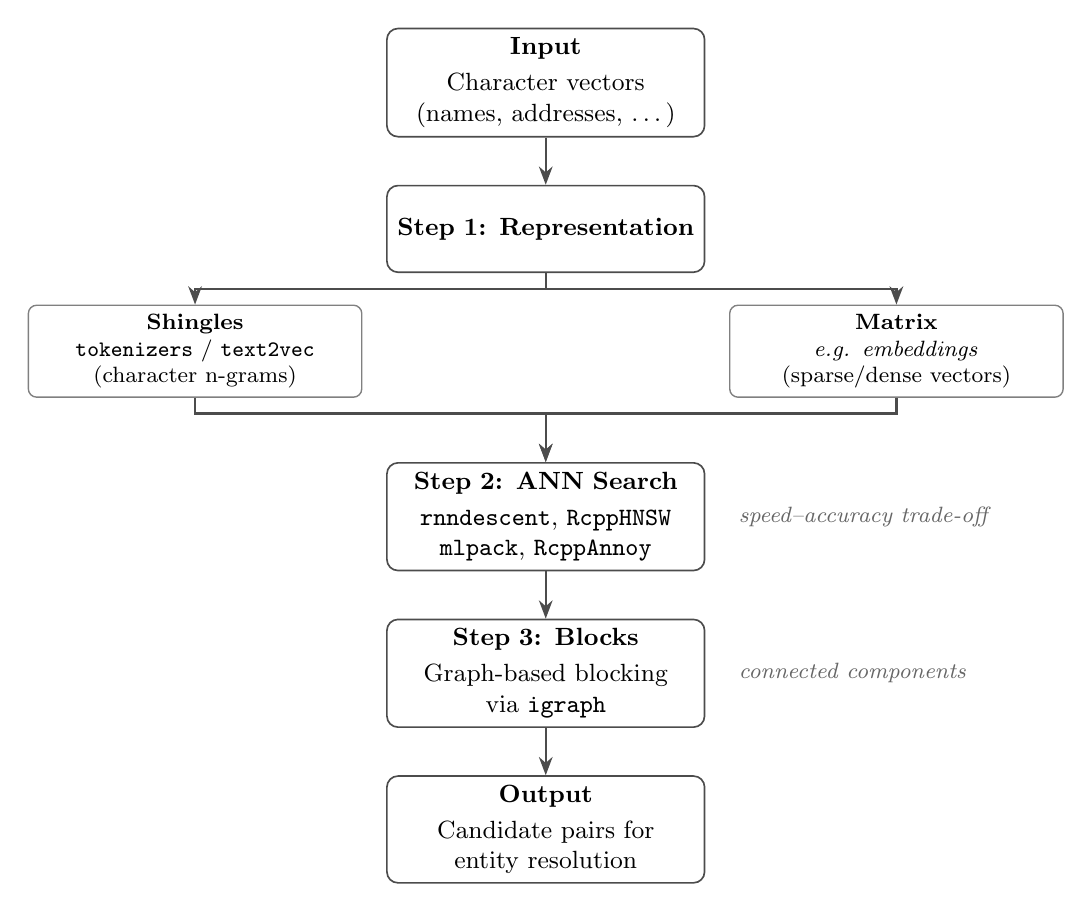
\begin{tikzpicture}[
  font=\small,
  box/.style={
    rectangle, rounded corners=4pt,
    draw=black!70, fill=white,
    text width=3.8cm, align=center,
    minimum height=1.1cm,
    line width=0.6pt
  },
  subbox/.style={
    rectangle, rounded corners=3pt,
    draw=black!50, fill=white,
    text width=4cm, align=center,
    minimum height=0.75cm,
    font=\footnotesize,
    line width=0.5pt
  },
  arrow/.style={
    -Stealth, line width=0.8pt, draw=black!70
  },
  label/.style={
    font=\footnotesize\itshape, text=black!60
  },
  >=Stealth
]

%% Step 1: Input
\node[box] (input) {%
  \textbf{Input}\\[2pt]
  Character vectors\\
  (names, addresses, \ldots)
};

%% Step 2: Representation
\node[box, below=0.6cm of input] (repr) {%
  \textbf{Step 1: Representation}
};

\node[subbox, below left=0.4cm and 0.3cm of repr] (shingles) {%
  \textbf{Shingles}\\
  \texttt{tokenizers} / \texttt{text2vec}\\
  (character n-grams)
};

\node[subbox, below right=0.4cm and 0.3cm of repr] (embed) {%
  \textbf{Matrix}\\
  \textit{e.g. embeddings}\\
  (sparse/dense vectors)
};

%% Step 3: ANN search
\node[box, below=2.4cm of repr] (ann) {%
  \textbf{Step 2: ANN Search}\\[2pt]
  \texttt{rnndescent}, \texttt{RcppHNSW}\\
  \texttt{mlpack}, \texttt{RcppAnnoy}
};

%% Step 4: Blocking
\node[box, below=0.6cm of ann] (blocks) {%
  \textbf{Step 3: Blocks}\\[2pt]
  Graph-based blocking\\
  via \texttt{igraph}
};

%% Step 5: Output
\node[box, below=0.6cm of blocks] (output) {%
  \textbf{Output}\\[2pt]
  Candidate pairs for\\
  entity resolution
};

%% Arrows
\draw[arrow] (input) -- (repr);
\draw[arrow] (repr.south) -- ++(0,-0.2) -| (shingles.north);
\draw[arrow] (repr.south) -- ++(0,-0.2) -| (embed.north);
\draw[arrow] (shingles.south) |- ++(0,-0.2) -| (ann.north);
\draw[arrow] (embed.south)    |- ++(0,-0.2) -| (ann.north);
\draw[arrow] (ann)    -- (blocks);
\draw[arrow] (blocks) -- (output);

%% Side annotations
\node[label, right=0.3cm of ann]    {speed--accuracy trade-off};
\node[label, right=0.3cm of blocks] {connected components};

\end{tikzpicture}

\end{document}
